\chapter{Rozbor řešené problematiky} 
\label{teorie}

Tato kapitola se věnuje teoretickému popisu jednotlivých částí systému. V průběhu jsou rozebírány i případné problémy, se kterými je potřeba se vypořádat. Jejich řešení je pouze nastíněno, samotná implementace je v kapitole \ref{implementace}. 

Prvním okruhem zájmu je způsob získávání dat z webu a jejich uložení. Dále se provede jejich analýza. Informace získané z analýzy je nutné také uložit a vhodným způsobem zobrazit uživateli (například jako tabulku nebo graf). Každému z těchto okruhů je věnována vlastní sekce. 

\section{Analýza sentimentu}
V této sekci chci rozebrat základní principy a metody analýzy sentimentu. Tato analýza se snaží v textu hledat názory uživatele a určit, jestli jsou pozitivní, negativní nebo neutrální. Názory se mohou týkat produktu, služby nebo například organizace jako celku, ale také jen jednotlivých částí. Analýza sentimentu se také zabývá extrakcí emocí z textu (hněv, radost, smutek). Názory jsou obvykle emocionálně zabarvené, to napomáhá je vyhledat. Emočně zbarvený text bude pravděpodobně obsahovat slova jako \uv{krásný} nebo \uv{příšerný}. Na základě tohoto faktu staví některé techniky analýzy. Objektivní komentáře typu \uv{Film je dlouhý 120 minut} nejsou pro tuhle analýzu zajímavé.

Výsledkem analýzy tedy může být polarita (pozitivní, negativní, popřípadě neutrální), někdy také doplněna intenzitou dané polarity (škála hodnot, například od 1 do 5).

Jak je popsáno v \cite{veselovska-2017}, analýza postoje se obecně dělí do třech úrovní. První analyzuje dokument jako celek (např. celý komentář), druhá úroveň je větní, která zjišťuje názor v~jednotlivých větách a třetí je na úrovni aspektu.
Analýza na každé z těchto úrovní obvykle vyžaduje trochu jiný přístup, některé metody analýzy jsou však využitelné na více úrovních. 

Analyzování na úrovni dokumentu je vhodné provádět pokud se celý dokument vyjadřuje k jedné entitě (v případě recenzí je to daný film). Analýza se provádí za předpokladu, že daný dokument obsahuje názor.

Na úrovni větní se zjišťuje jaký sentiment mají jednotlivé věty, to dává větší detail o~analyzovaném textu. Sloučením sentimentů jednotlivých vět je možné zjistit celkový sentiment dokumentu. Analýza na této úrovni souvisí s analýzou subjektivity, která rozpoznává objektivní věty od subjektivních (některé věty názor neobsahují a jak už bylo řečeno, objektivní věty nejsou pro analýzu zajímavé). Polarita názoru se tedy analyzuje až poté, co je věta označena za subjektivní. Objektivní věty se obvykle označují za neutrální. 

Analýza na úrovni aspektu sleduje názory na určité části dané věci. Například ve větě \uv{Herci byli skvělí, ale prostředí nic moc.} se vyskytují dva aspekty filmu. Herci, ti mají hodnocení pozitivní a prostředí, které má negativní. Analýza na úrovni aspektu se dělí na dva úkoly. Prvním je nalezení zmínky o hledaném aspektu a druhým je přiřazení polarity této zmínce.

Analyzovat postoj uživatele není jednoduchý úkol. Velkou problematiku přináší lidský jazyk, který je dosti volný a kontextový. Jedním z těchto problémů je rozpoznat ironii a~sarkasmus. 
Například z věty \uv{Tento film je opravdu výborný!} nelze poznat, jakým způsobem to autor myslel.
Jak popisuje \cite{filatova-2012-irony}, nejzásadnější komplikací je fakt, že ironie ani sarkasmus nejsou formálně definovány a nedají se lehce poznat (například sadou pravidel). Oba tyto fenomény jsou dynamické a vyvíjí se. Ironii a sarkasmus se dá částečně poznat podle některých ustálených frází, emotikonů nebo například otazníků a vykřičníků. Dalším pomocným faktem je, že ironie a sarkasmus se častěji využívají pro záporná hodnocení a často se objevují v podobném kontextu. Ocitovaná práce se problém sarkasmu a ironie snaží řešit vytvořením párů ironických a neironických recenzí ke stejnému produktu a jejich následnou analýzou.

Zde \cite{Ptcek2014SarcasmDO} tento problém řeší využitím klasifikátorů založených na metodě pomocných vektorů a maximální entropie. Klasifikátory jsou trénovány na datech ze sociální sítě \emph{Twitter}. V práci jsou prozkoumány různé metody předzpracování a extrakce příznaků, snaží se také zpracovat emotikony a interpunkční znaménka. Vytvořený systém detekuje ironii a~sarkasmus s F1 skóre 0.92 pro angličtinu a 0.58 pro češtinu. Tento rozdíl je způsobený velikostmi trénovacích datových sad (trénovací sada pro angličtinu je mnohem větší). Při zmenšení anglické datové sady na velikost české klesne F1 skóre klasifikátoru pro angličtinu pouze na 0.73, z toho vyplývá, že v českém jazyku je obtížnější detekovat ironii a sarkasmus.  

V následujících podsekcích rozebírám základní metody analýzy. Podle \cite{approaches} (práce byla využita pro základní informace o metodách) jsou přístupy založené na slovníku, pravidlech nebo strojovém učení.


\subsection{Metody využívající lexikon}
Základem metod je myšlenka, že celková polarita věty nebo dokumentu se dá zjistit z~polarit jednotlivých slov nebo frází. Má více možných implementací, obecně je však analýza založena na seznamu slov (frází), které jsou označeny polaritou a jejich intenzitou. Slovo \uv{děsný} by mělo například hodnotu -7 (polarita záporná s intenzitou 7). Naopak slovo \uv{úžasný} by mělo například hodnotu 6 (polarita kladná s intenzitou 6). 
Jakou polaritu a intenzitu by slova měly mít jsou problémy samy o sobě. Polarita je závislá na kontextu (\uv{malý pokoj v~hotelu} versus \uv{malá čekací doba}). Určení intenzity je zase silně subjektivní, každý má k určitým slovům různé asociace.

Například v \cite{lexikon} je tato metoda dále rozšířena o sledování intenzifikace (\uv{docela dobrý} versus \uv{velice dobrý}) a negace (\uv{je dobrý} versus \uv{není dobrý}). Takovýchto rozšíření této metody existuje celá řada.

Přesnost metody využívající lexikon je oproti ostatním metodám více závislá na správném předzpracování dat. Normalizace, lemmatizace a stematizace velice napomáhají v přiřazení slov z textu k těm, které se vyskytují v předem vytvořeném lexikonu.

Po sestavení dostatečně velkého lexikonu nejčastěji používaných slov se vezme analyzovaný text a všem slovům se přiřadí jejich hodnota z lexikonu. Slova bez polarity (předložky, spojky apod.) se v lexikonu nenachází. Poté se jen sečtou všechny hodnoty a tím vznikne výsledné hodnocení daného textu. Výsledná hodnota se vydělí počtem slov v textu. Tímto se celkové ohodnocení textu normalizuje a předejde se tomu, že by text byl pozitivnější jenom protože je delší. 

\subsection{Metody založené na pravidlech}
Podle definice v \cite{approaches}, metoda využívá člověkem předem definovaných pravidel. Nejprve se celý dokument rozdělí na slova. Poté se podle daných pravidel testuje přítomnost slov, které jsou opět uložené v lexikonu. Stejně jako u metody založené na lexikonu se připočítává celkové skóre dokumentu. Pokud je celkové skóre větší nebo rovno nula je dokument pozitivní, pokud menší než nula, je dokument negativní. Výstup analyzátoru se porovná se správnou odpovědí. Pokud v lexikonu analyzátoru chybí nějaká slova z textu, která by napomohla analýze, jsou přidána do lexikonu. Analyzátor je tak schopný učit se nová slova ze vstupního textu.

\subsection{Metody založené na strojovém učení}
\label{machinelearning}
Těchto metod opět existuje celá řada \cite{approaches} \cite{MEDHAT20141093}, každá s různými implementacemi. 
Základní myšlenka je vytvoření algoritmu, který je schopný ze vstupních dat vytvořit správná výstupní data bez toho, aby bylo explicitně naprogramováno, jak to má udělat. 

Tohoto jsou algoritmy schopny dosáhnout za pomocí učení (trénování). Učením je zde myšleno upravování vnitřních proměnných modelu na základě vstupů tréningových dat. Vstupním datům se také říká vektor příznaků (vstupní dokument), který se skládá z jednotlivých příznaků (slov). Mimo analýzu sentimentu mohou příznaky být například hodnoty pixelů obrázku, celá nebo desetinná čísla jakýchkoliv hodnot, popřípadě pravděpodobnosti. Každá metoda strojového učení se trénuje trochu jiným způsobem, základní myšlenka úprav vnitřních proměnných modelu však zůstává.

Mezi jedny z nejpoužívanějších algoritmů strojového učení pro analýzu sentimentu patří metody podpůrných vektorů (angl. \emph{support vector machines}), pravděpodobnostní modely a~hluboké učení.

Jak popisuje \cite{svm}, \textbf{metoda podpůrných vektorů} funguje na principu rozdělení $N$~rozměrného~prostoru vstupních příznaků pomocí nadroviny. V případě analýzy sentimentu je prostor obvykle rozdělen lineárně pro zamezení přeučení. Každé slovo v tomto prostoru představuje jeden rozměr. Počet slov v daném textu pak představuje hodnotu v tomto rozměru. Určitý text je tedy reprezentován bodem v prostoru, jeho souřadnice jsou určeny slovy a počtem těchto slov.
Trénování při využití tohoto algoritmu spočívá v nalezení správného rozdělení na podprostory (například jeden podprostor pro pozitivní a jeden pro negativní sentiment) podle shluků pozitivních a negativních textů (bodů). 

Po procesu trénování je analyzovaný text namapován do vytvořeného prostoru, podle toho v jakém podprostoru skončí je jeho sentiment prohlášen za pozitivní nebo negativní. 


\textbf{Pravděpodobnostní modely} \cite{prob1} \cite{prob2} předpovídají pravděpodobnosti všem možným výstupům na základě současného vstupu a předchozí tréningové sadě. Výstup s nejvyšší pravděpodobností je prohlášen za správný.

Mají hned několik výhod. Jednou z nich je jednoduchost, to znamená, že jim stačí malá tréningová sada a rychle se trénují (oproti například neuronovým sítím). Další výhodou je poměrně velká přesnost, a to i když jsou trénovány na malém počtu dat. Neposlední výhodou je fakt, že mimo výslednou polaritu vrací i jistotu dané předpovědi. Obvykle se tedy využívají tam, kde je menší tréningová sada, není potřeba až tak vysoká přesnost nebo je potřeba mít rychle natrénovaný model. Neuronové sítě v porovnání potřebují více tréningových dat a více času na trénování, ale jsou přesnější.

Pravděpodobnostních modelů  a jejich implementací je samozřejmě několik. Nejznámější z nich je naivní Bayesův klasifikátor, proto se na něj chci nyní zaměřit.

Klasifikátor se může lišit podle toho, jaká je využita implementace a s jakými daty pracuje. Například při práci s výškou lidí by se muselo vzít v potaz rozložení výšky lidské populace. To se řídí normálním rozložením, takže při výpočtu pravděpodobností se využije právě vzorec pro normální rozložení. Při práci s textem stačí pouze počítat výskyty slov.

Klasifikátor potřebuje tréningová data obsahující vstupní příznaky i hledaný výstup pro vymodelování pravděpodobností.

Již podle názvu klasifikátoru se dá zjistit, že pracuje na základě Bayesovy věty. Jak přesně ji využívá popisuji dále. Naivní je, protože je pro něj každé slovo nezávislé na ostatních. Nepracuje tedy s větami, ale se seznamem individuálních slov.
Jak popisuje \cite{prob1} předpoklad by byl, že přesnost kvůli naivitě nebude moc velká, ale praktické výsledky ukazují opak.

Bayesova věta:
\begin{equation}
  P(A|B)=\frac{P(B|A)\cdot P(A)}{P(B)}
  \label{eq:rovnice1}
\end{equation}

Pro výpočet klasifikace se za $B$ dosadí vstupní seznam příznaků a za $A$ se postupně dosazují jednotlivé možné výstupy klasifikace. Výstupní třída s nejvyšší pravděpodobností je prohlášena za správný výstup klasifikátoru. Protože se pro výpočty pravděpodobností jednotlivých výstupů liší pouze čitatele zlomku, jmenovatele jsou vynechány. Na výsledku to nic nezmění (pouze porovnáváme která pravděpodobnost je vyšší).

Po dosazení by to tedy mohlo vypadat takto(pos je označení pro pozitivní sentiment, neg je označení pro negativní sentiment):
\begin{equation}
  P(pos|Film\:byl\:super)=P(Film\:byl\:super|pos)\cdot P(pos)
\end{equation}

\begin{equation}
  P(neg|Film\:byl\:super)=P(Film\:byl\:super|neg)\cdot P(neg)
\end{equation}

$P(pos)$ a $P(neg)$ jsou pouze poměry výskytů jednotlivých tříd v trénovací sadě. Teď už tedy stačí vypočítat $P(Film\:byl\:super|pos)$ a $P(Film\:byl\:super|neg)$. V podstatě by stačilo spočítat kolikrát se v tréningové sadě vyskytuje věta \uv{Film byl super} pod třídou pos a~kolikrát pod třídou neg. Problémem je, že věta se nemusí v tréningové sadě vůbec objevit. Tento problém řeší naivita klasifikátoru. Pravděpodobnost věty se rozdělí na násobek pravděpodobností jednotlivých slov:

\begin{equation}
  P(Film\:byl\:super)=P(Film) \cdot P(byl) \cdot P(super)
\end{equation}

Pravděpodobnost jednotlivých slov se vypočítá:
\begin{equation}
  P(Film|pos)=\frac{x}{y}
\end{equation}
Kde $x$ je počet výskytů slova "Film" v textech třídy pos a $y$ je počet všech možných slov ve třídě pos.
Tohle samozřejmě jen přesune daný problém z vět na slova, dané slovo se nemusí objevit v trénovací sadě. To by nám dalo pravděpodobnost slova $0$ a protože násobíme, pravděpodobnost celé věty by byla také $0$. Problém se dá obejít využitím Laplaceova vyhlazování. Ke každému výskytu přičteme $1$, aby nikdy nebylo $0$ a ke jmenovateli přičteme počet všech unikátních slov přes obě třídy (aby pravděpodobnost nebyla větší než $1$).

Tímto se vytvoří tabulka, kde ke každému slovu vyskytujícímu se v trénovací sadě jsou přiřazeny pravděpodobnosti každé třídy (pos a neg). 
Při analýze stačí jen vynásobit pravděpodobnosti slov vyskytujících se v analyzované větě. Samozřejmě jednou se násobení provede pro třídu pos a po druhé pro třídu neg. Porovnáním výsledných pravděpodobností násobků se zjistí, která odpověď je pravděpodobnější.


\textbf{Hluboké učení} je dnes největší novinkou nejen při analýze sentimentu \cite{survey} \cite{survey2}.

\begin{figure}[!htb]
\centering
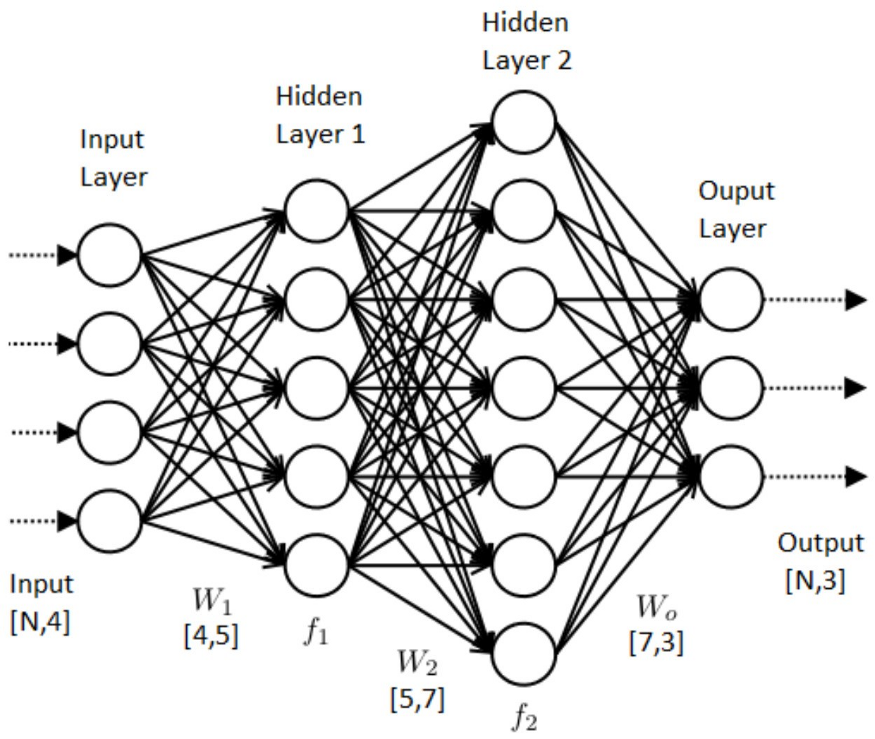
\includegraphics[width=\textwidth/2]{neural_network.png}
\label{neuronovasit}
\caption{Obrázek neuronové sítě. $N$ značí vstupní a výstupní neurony, $W$ značí váhy spojů mezi neurony a $f$ jsou \uv{výpočetní} neurony. Převzato z \url{https://medium.com/coinmonks/the-artificial-neural-networks-handbook-part-1-f9ceb0e376b4}}
\end{figure}

 Využívá se k řešení problémů, které nebylo možné dříve vyřešit (například klasifikace obrázků, rozpoznání slov z lidské řeči a podobně). Neustále se nachází nová využití pro tuto metodu (od překládání jazyků v reálném čase po řízení automobilů).
V oblasti analýzy sentimentu je tato metoda také přelomová. Za správných podmínek dosahuje nejvyšší přesnosti ze všech algoritmů, je však doménově závislá a náročná na trénování.


Koncept je poměrně starý, počátky již v padesátých letech minulého století. Trénování neuronových sítí je výpočetně velice náročné a potřebují velké množství tréningových dat, proto je rozvoj možný až nyní díky výkonnější výpočetní technice (převážně grafickým kartám) a přístupu k obrovskému množství dat. 

Jako spousta dalších algoritmů (hejno částic, mravenčí kolonie a například genetický algoritmus) je i tento inspirován přírodou.
Hluboké učení se snaží napodobit funkci biologického mozku. Neuronová síť je složena z množství neuronů a spoji mezi nimi viz. obrázek~\ref{neuronovasit}. 
Jako v biologickém mozku, každý neuron je schopný zpracovat signál a poslat ho pomocí spojů (synapsí) dalším neuronům. Neuron je v tomto případě vlastně jen obyčejná sčítačka. Všechny vstupy do neuronu jsou vynásobeny váhou daného spoje a sečteny. K~tomuto výsledku se obvykle ještě přičte práh. Po přičtení prahu je použita aktivační funkce (například \emph{sigmoid}, \emph{tanh} nebo \emph{ReLu}) a výsledek je výstupními spoji poslán dalším neuronům. 
Hodnoty prahů a vah spojů jsou z počátku nastaveny náhodně a v průběhu trénování se upravují. 


Hluboké učení je využití neuronových sítí v několikavrstvé architektuře. Architekturu je samozřejmě možné zapojit více způsoby. Pro analýzu sentimentu se nejvíce používají následující architektury neuronových sítí:

\begin{itemize}
    \item Rekurentní - Třída neuronových sítí, kde jednotlivá propojení mezi neurony tvoří cyklus. Každý cyklus je tvořen jednou vrstvou neuronů. Oproti klasické dopředné neuronové síti má vnitřní paměť. Je tedy vhodná ke zpracování sekvenčních dat (mimo jiné i textu). V paměti je uložen aktuální stav zpracování, tento stav je upravován každým příchozím slovem. Stav má tedy uchováno vše, co se postupně zpracovalo. Tento typ neuronových sítí trpí problémem mizejícího a explodujícího gradientu, toho se snaží vyvarovat úpravy této architektury (obousměrné anglicky \emph{bidirectional} architektury a~\emph{LSTM}). 
    \item \emph{LSTM} (\emph{long short term memory}) - Je speciálním typem rekurentní neuronové sítě, která řeší problém mizejícího gradientu. Oproti rekurentní síti má každý cyklus čtyři vrstvy neuronů, které mezi sebou komunikují. Navíc má dva vnitřní stavy místo jednoho. Jednotlivým vrstvám se říká brány a jsou následující: \uv{zapomínající}, \uv{pamatující}, \uv{vstupní} a \uv{výstupní}. Problém mizejícího gradientu je vyřešen kombinací těchto bran a využitím jednoho vnitřního stavu navíc.
    \item Rekurzivní - Tento typ neuronových sítí se obvykle využívá ke zpracování dat v acyklickém grafu (stromu). Je vlastně generalizací rekurentních neuronových sítí. Neuronová síť postupně prochází stromovou strukturu od listů směrem ke kořenu a vytváří rodičovské uzly kombinací jednotlivých tokenů. 
\end{itemize}

Učení neuronových sítí je možné provádět s učitelem, bez učitele a zpětnovazební. Zpětnovazební učení se při analýze sentimentu nevyužívá, proto se na něj nebudu zaměřovat.  

\textbf{Učení s učitelem} je proces při kterém je model učen hledat k danému vstupu korektní výstup. Model tedy hledá funkci $f$ takovou, která bude mít správný výstup $f(x)$ pro co nejvíce vstupních vzorků $x$. Pokud se hledá konkrétní třída z předem dané množiny hovoříme o klasifikaci, pokud se hledá hodnota v určitém rozsahu mluvíme o regresi. Korektní výstupy jsou předem definovány lidmi. Je potřeba mít dostatečně velký počet trénovacích dat, které obsahují vstup a k němu hledaný výstup. Toto může být problematické, protože vytvoření takto označených dat není jednoduché, někdy nemožné. 

V případě analýzy sentimentu bude vstupem text a výstupem hledaný sentiment (pozitivní nebo negativní, popřípadě třídy hodnot). Takto označená data se předají modelu, který se na základě textu pokusí předpovědět výstup (na začátku procesu trénování pravděpodobně chybně). Předpověď je poté porovnána se správnou odpovědí. Porovnání je prováděno tak zvanými ztrátovými funkcemi. Ztrátových funkci je několik, každá se používá pro řešení jiného problému.


Podle chybovosti se modelu upraví proměnné (váhy spojů a hodnoty prahů), aby byl příště přesnější (využívá se derivací pro zjištění správné úpravy). Po dostatečně dlouhém trénování se model naučí potřebné generalizace k tomu, aby byl schopný předpovídat korektně výstup i na datech, které ještě před tím nikdy neviděl.
 
\textbf{Učení bez učitele} využívá pro trénování pouze vstupy \cite{machinelearning}. Hledaný výstup není označen. Analyzátor se snaží ve vstupních datech nalézt strukturu dat a vztahy mezi jednotlivými příklady. Výstupem bývají shluky, kolem kterých se data pohybují. Všechna přiložená data při tréningu se tak strukturují a je možné v nich nalézt podobnosti. 

Podle \cite{unsupervised} je možné pro analýzu sentimentu využít učení bez učitele následujícím způsobem. Využívá se faktu, že negativní nebo pozitivní slova bývají vždy obklopena podobnými slovy. Například slovo \uv{dobrý} je vždy obklopeno obdobnými slovy jako slovo \uv{úžasný}. Tímto způsobem se vytvoří shluk pozitivních a shluk negativních slov. Podle vzdálenosti od středu daného shluku je možné zjisti jak moc pozitivní / negativní dané slovo je. Postupně tak můžeme ohodnotit pozitivitu celého textu.



\section{Pokročilé metody zpracování přirozeného jazyka}
Tato kapitola nabízí přehled novějších technik, technologií a systémů. Základní myšlenka konceptu hlubokého učení je spolu s dalšími základními algoritmy strojového učení popsána v kapitole \ref{machinelearning}. Na základním konceptu hlubokého učení staví mnoho dalších technologií, které zde budou popsány. Samozřejmě existují nové techniky, technologie a systémy, které hlubokého učení nevyužívají. Z osobního zájmu (technologie hlubokého učení mi přijdou zajímavé) se ale soustředím právě na ně. Základní přehled existujících technologií byl nalezen v \cite{survey}.


\subsection{Vnoření slov}
Anglicky známé jako \emph{word embedding}. Vnoření slov je technika jazykového modelování a~reprezentace příznaků. Slova ze slovníku jsou převedena na vektor desetinných čísel. Tento vektor je obvykle vytvořen převedením z řídkého vektoru 1 z $N$ (anglicky \emph{one-hot vector}). Převedený vektor již není řídký, obsahuje nenulové hodnoty ve všech dimenzích (pokud tedy určitá hodnota v dimenzi není reprezentována právě nulou). Zároveň je dimenzí mnohem méně. 

Základní myšlenkou této reprezentace je, že každá dimenze nově vytvořeného vektoru představuje nějakou vlastnost daného slova, podobná slova tedy budou mít podobné číselné reprezentace. Zajímavostí takto vytvořených číselných reprezentací jsou výsledky po matematických operacích mezi slovy. Vlastnost je často vysvětlena následujícím příkladem. Když se vezme vytvořená vektorová reprezentace pro slovo \uv{král}, odečte se od ní vektor slova \uv{muž} a přičte vektor slova \uv{žena}, výsledkem by měla být vektorová reprezentace podobná slovu \uv{královna}.


Vnoření slov je možné využitím hlubokého učení implementovat například metodami \emph{CBOW} \cite{cbow} (\emph{continuous bag of words}), SG \cite{sg} (\emph{Skip-Gram}) a GloVe (\emph{Global Vector}). Metody \emph{CBOW} a \emph{SG} jsou dnes implementovány pod populárním systémem zvaným \emph{Word2Vec}. Tento systém využívá vlastností obou metod pro co nejlepší výsledky. Metoda \emph{CBOW} je přesnější pro menší datové sady, naopak \emph{SG} je přesnější trénováním na větších datových sadách.

Obě metody trénují neuronové sítě velice podobným způsobem. Trénovací data není potřeba anotovat. Metoda \emph{CBOW} učí neuronovou síť předpovědět slovo podle jeho kontextu (kontext je vstupem a slovo výstupem). Naopak metoda \emph{SG} předpovídá kontext podle daného slova (slovo je vstup, kontext výstup). Jeden trénovací příklad by tedy mohl vypadat dle obrázku \ref{trainexample}.

\begin{figure}[!htb]
\centering
\label{trainexample}
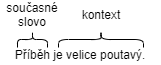
\includegraphics[width=\textwidth/4]{cbow_sg_example.png}
\caption{Ukázka trénovacího příkladu.}
\end{figure}




\subsection{Mechanismus pozornosti pro neuronové sítě}
Tato technika pomáhá řešit problém se vzdálenými závislostmi v sekvenci dat (například závislost mezi prvním a posledním slovem ve větě). Tento problém se snaží řešit oboustranné rekurentní neuronové sítě a LSTM sítě, v praxi je to však stále problematické. 

Tento mechanismus je inspirován vizuální pozorností lidí. Stejně jako lidský zrak se tato metoda soustředí na určitou část ve vysokém rozlišení a okolí je v nízkém rozlišení. Část pod vysokým rozlišením se postupně posouvá v čase. Mechanismus pomáhá trénovanému modelu naučit se které části dat věnovat pozornost na základě vstupu a současného stavu zpracování dat. 


Mechanismus byl například využit v systému pro překlad mezi jazyky \cite{Bahdanau2015NeuralMT}. Pozornost byla využita pro výběr slov relevantních při překladu. Model se postupně soustředí na jednotlivé části překládané věty. Samozřejmě nestačí jít slovo po slovu, protože jazyky často vyjadřují stejnou věc jiným počtem slov. Model se tedy musí naučit toto mapování. Například při překladu z angličtiny do francouzštiny se slovo \emph{destruction} překládá jako \emph{la destruction}, to znamená, že při překladu jednoho slova v angličtině se musí soustředit na vytvoření dvou slov ve francouzštině. 

\subsection{Paměťová síť}


%https://arxiv.org/abs/1410.3916
Anglicky známé jako \emph{memory networks}. V této práci \cite{Weston2015MemoryN} byla síť představena jako systém schopný přijímat logická tvrzení a podle nich poté odpovídat na otázky. Systém je složen z~několika komponent. Jednou z těchto komponent je paměťová část. Paměťová část je oproti například rekurentním neuronovým sítím mnohem větší a dlouhodobější. Jednotlivé části mohou být implementovány jako neuronové sítě, v práci byly prozkoumány i další metody. Paměťová část se chová jako dynamické úložiště znalostí získaných z jednotlivých tvrzení. 
Ostatní komponenty jsou následující:
\begin{itemize}
    \item I (\emph{input feature map}) - převede příchozí data do vnitřní reprezentace
    \item G (\emph{generalization}) - zpracovává příchozí informace (tvrzení), upravuje podle nich paměť znalostí. Má schopnost zestručnit a zobecnit všechny získané znalosti. 
    \item O (\emph{output feature map}) - z již získaných znalostí a nového vstupu vytváří nový výstup. Výstup je stále ve formátu vnitřní reprezentace.
    \item R (\emph{response}) - převádí výstup z vnitřní reprezentace do požadovaného formátu, například text nebo akce.
\end{itemize}

Síť nejprve dostane několik vět a poté otázku, na kterou má odpovědět. Systém je schopný nalézt ve větách potřebné informace a podle nich vytvořit odpověď. Komponenta I přečte jednotlivé věty a přeloží je do vnitřní reprezentace sítě. Poté komponenta G upraví paměť podle nově získaných informací. Po zpracování všech vstupních vět jsou věty uloženy do matice vět. Otázka je také nejprve převedena do vnitřní reprezentace, poté komponenta O nalezne potřebné informace ve vnitřní paměti a vytvoří odpověď. Nakonec je odpověď převedena komponentou R.


\subsection{BERT}

Je zkratka z anglického \emph{\textbf{B}idirectional \textbf{E}ncoder \textbf{R}epresentations from \textbf{T}ransformers}, byl vytvořen společností Google pro lepší pochopení uživatelských vyhledávání \cite{bert}. Tento systém má za cíl naučit se modelovat (dá se říci \uv{pochopit}) jazyk. Technická inovace spočívá ve využití oboustranného trénování transformerů (z anglického \emph{transformer}), což jsou modely využívající koncept pozornosti. Předchozí systémy se obvykle na text dívaly jako na sekvenci slov jdoucí zleva doprava, popřípadě v kombinaci s pohledem zprava doleva. Výsledky systému \emph{BERT} však ukazují, že modely trénované oboustranně mají hlubší pochopení kontextu a sekvencí slov. Vstupní sekvence slov se čte jako celek, to napomáhá modelu se naučit kontext určitého slova na obou stranách. Trénování modelu probíhá následujícími metodami:
\begin{itemize}
    \item maskováním slov - Před předáním trénovací sekvence slov modelu se nahradí 15 \% slov maskovacím tokenem. Model se poté učí předpovědět maskovaná slova podle ostatních slov v sekvenci. 
    \item předpovídáním následující věty - Model postupně dostává dvojice vět. Polovina dvojic vět na sebe navazuje, druhá polovina ne. Model se učí předpovídat jestli druhá věta patří za první či nikoliv. 
\end{itemize}

Model dále využívá toho, že je předem natrénovaný na obrovské sadě dat. Při vytváření modelu pro nový úkol se obvykle musí natrénovat od úplného počátku, to může trvat i~desítky hodin. Tento problém řeší právě předem natrénovaný \emph{BERT}, který pro specifický úkol stačí doladit \cite{finetune}. Autoři systému doporučují dolaďování dvěma až čtyřmi epochami, \emph{BERT} byl v porovnání trénován stovky hodin.    

\emph{BERT} se dnes využívá na množství úkolů zpracování přirozeného jazyka, ve velkém počtu z nich má nejlepší výsledky. Například na těchto stránkách\footnote{\url{http://nlpprogress.com/english/sentiment_analysis.html}} lze vidět všechny jeho využití.


\section{Získání dat z webových portálů}
\label{stahovani}
Před samotným získáním dat je dobré vědět kolik a jakých dat bude potřeba. Proto je vhodné nejprve prozkoumat metody analýzy. Z porovnání metod \cite{approaches} je patrné, že největší přesnost mají analyzátory využívající strojové učení. Z tohoto důvodu bych se přikláněl k~využití těchto analyzátorů. Jejich nevýhodou je nutnost trénování.

Jak je napsáno na tomto blogu \cite{dataamount}, při vytváření analyzátoru na bázi umělé inteligence/strojového učení je potřeba obrovské množství dat pro jeho trénování. O trénování a analýze jsem již psal, nyní stačí informace, že budou potřeba data pro trénování analyzátoru. Těchto dat by mělo být co nejvíce, protože čím větší vzorek dat je použit, tím více vzorů vyjadřování se analyzátor naučí a poté je při samotné analýze přesnější.

Dalším důvodem, proč je potřeba velké množství dat je mimo trénování samotná analýza. Z velkého počtu názorů je patrnější celkový názor na produkt a je pravděpodobnější získat více pohledů na věc.

Z předchozí analýzy tedy vyplynulo, že bude potřeba co nejvíce dat, tato data je možné získat z internetových stránek. Na internetu je velké množství uživatelů a všichni nějakým způsobem přispívají k jeho obsahu \cite{useramount}. Konkrétní počet uživatelů na internetu pro rok 2019 je 4,4 miliard, takové množství uživatelů je schopné vyprodukovat obrovské množství dat každou minutu, konkrétní čísla pro největší sociální média jsou na citovaném blogu.

Uživatelé přispívají na sociálních médiích, speciálních stránkách určených pro recenze nebo přímo na stránkách prodejců. Díky tomu je vytvářeno obrovské množství nestrukturovaných dat, které je možné využít pro analýzu názorů na téměř jakékoliv téma.

Mimo kvantitu dat je také důležitá jejich kvalita. Pokud je analyzátor trénován na špatných datech, nedá se předpokládat, že by měl velkou přesnost. Zpracování dat pro zvýšení jejich kvality je popsáno v kapitole \ref{predzpracovani}. Data (obzvlášť ta stažená z internetových diskuzí) nejsou vždy validní. V případě filmové recenze může být napsána člověkem, který prostě nemá daný žánr rád, nebo může jít o \emph{internetového trolla} \cite{televize}. Ve zkratce, internetový troll je někdo, kdo se snaží narušit věcnou konverzaci nad tématem. Obvykle se snaží z~ostatních uživatelů dostat emocionální reakci.
Validita příspěvku se však nedá jednoduše poznat, proto se musí předpokládat, že každý příspěvek je svým způsobem validní (každý má svůj názor, který se musí vzít v potaz). Při výsledné analýze nevalidní příspěvky příliš nevadí (s nimi se obvykle počítá). Všechny názory jsou důležité, protože utváří celkový pohled na daný film. Pro společnosti je vhodné sledovat všechny názory, aby věděli jakým směrem se dále ubírat, nevalidní příspěvky však při trénování analyzátoru mohou zhoršit jeho přesnost. Validita příspěvků se na některých webech dá poznat pomocí hodnocení (\uv{lajků}) od ostatních uživatelů (tato možnost však není vždy).  

Pro získání dat z webových stránek je hned několik možností. Některé webové stránky mají své rozhraní pro programování aplikací (z anglického application programming interface, zkratka API), pomocí kterého lze požadovaná data získat. Jak píše \cite{webscraping}, API je část serveru odpovědná za přijímání a odesílání požadavků a dat. K tomu jsou obvykle využívány metody GET nebo POST. 

Data jsou odeslána v předem domluveném formátu jako například JSON. Na rozdíl od klasického webového serveru tedy neodesílá HTML dokument, ale pouze požadovaná data.
Při práci s API většinou stačí využít jeho konkrétní knihovnu nebo url adresu a jejich předdefinované funkce. Každá taková funkce má svou dokumentaci, je tedy jasné co funkce vyžaduje a co vrátí. Vše bývá již připraveno pro pohodlí uživatele, je tedy jednoduché se v datech zorientovat, poté je zpracovat a například uložit. Většina stránek však žádné API nemá, nebo k němu dávají přístup pouze ve speciálních případech na zažádání (k přístupu bývá potřeba speciální klíč).
Musí se tedy využít jiné nástroje. 

Obecně se získávání dat z webu mimo použití API říká \emph{web scraping} \cite{webscraping}. \emph{Web scraping} je soubor technik, které lze využít k získání požadovaných (obvykle nestrukturovaných) dat z webových stránek. Mezi tyto techniky patří způsoby pro nalezení hledaných dat i jejich samotné stažení a následné formátování. \emph{Web scraping} zahrnuje široký rozsah programovacích technologií mezi které patří například analýza dat, zpracování přirozeného jazyka a~zabezpečení informací.

Když se provádí automatizovaný \emph{web scraping}, webové stránky můžou být děleny do dvou typů. Stránky používající JavaScript pro vytváření (obvykle dostahování) obsahu, a~stránky bez něj. Při manuálním kopírování dat ze stránky přítomnost JavaScriptu proces neovlivňuje.

Stránky bez JavaScriptu jsou po přijetí požadavku serverem celé odeslány v těle HTTP odpovědi serveru jako HTML dokument. Proto pouze stačí poslat na server HTTP dotaz a~přijatý HTML dokument zpracovat podle potřeby. 

Stránky používající JavaScript pro doplnění obsahu fungují jinak. Nemusí vždy přímo obsahovat hledaná data. HTML dokument obsahuje základní kostru stránky a část dat. Zbylá data jsou načítána dynamicky pomocí skriptů, které se spouští až v prohlížeči uživatele.
Podle toho, jaká data uživatel potřebuje (na co klikl, jestli je přihlášený apod.) JavaScript zašle další požadavky na server. Této technologii se říká AJAX (zkratka z anglického asynchronous JavaScript and XML, neboli asynchroní JavaScript a XML).
Od serveru se vrátí potřebná data obvykle ve formátu JSON a stránka se z těchto částí dat seskládá až v prohlížeči. Proto není možné na server zaslat HTTP požadavek a obdržet zpět stejný HTML dokument jako ten vykreslovaný v prohlížeči.
Pro stahování z JavaScriptových stránek je možné využít \emph{Reverse Engineering} JavaScriptu nebo jeho \emph{Rendering}. \emph{Reverse Engineering} se dělá za pomoci sledování požadavků JavaScriptu a následného zaslání stejných požadavků. Přijatá data se následně seskládají do celku. Druhá metoda je vykreslení a zpracování požadované stránky za pomocí nástroje jako je Selenium. Tento nástroj využívá prohlížeč pro vykreslení stránky a vlastně simuluje návštěvu stránky uživatelem. Po vykreslení webové stránky stačí seskládaný HTML dokument zpracovat podle potřeby.

Jak je napsáno na \cite{shieldsquare} a \cite{jetruby} mezi konkrétní způsoby extrakce dat patří jejich manuální kopírování , \emph{HTML parsing}, \emph{DOM parsing}, využití \emph{XPath}, \emph{google sheets}, a \emph{text pattern matching}. 

Jednotlivé techniky stahování a extrakce hledaných dat jsou popsány v následujících podkapitolách.

\subsection{Manuální kopírování dat}
Anglicky se této technice říká \emph{copy-pasting}. Technika spočívá v prostém kopírování chtěných dat ze zdroje a jejich vkládáním do datového úložiště. Při větším objemu dat tato technika zabere mnoho času a úsilí, práce je velice repetitivní. Na druhou stranu je tato metoda jedinou použitelnou pokud je webová stránka pod ochranou proti stahovacím skriptům. Efektivní je také při získávání pouze malého množství dat. Vzhledem k tomu, jak je tato technika pomalá a neefektivní se moc nevyužívá. Všechny ostatní metody popsané níže jsou automatizované.

\subsection{\emph{HTML parsing}}
Obvykle se dělá za pomocí knihoven jako je například BeautifulSoup. Metoda spočívá ve stažení celého HTML dokumentu a jeho následném prohledání. Využívá se \emph{tagů} a stromové struktury HTML dokumentu. Před napsáním skriptu, který extrahuje hledaná data je nutnost znát stromovou strukturu HTML dokumentu i názvy klíčových uzlů stromu. Strom se poté postupně prochází a extrahují se hledaná data. Cílí na HTML stránky, lineární i~zanořené. Tato metoda je velice rychlá a jednoduchá. Využívá se pro extrakci textu, odkazů zdrojů (např. obrázků) a podobně.

\subsection{\emph{DOM parsing}}
\emph{Document object model} zkráceně DOM, definuje styl, strukturu, ale také obsah dokumentu. Tato technika je schopná získat podrobný pohled na strukturu stránky. Skripty mohou nalézt uzly dokumentu, které obsahují potřebná data a poté pomocí nástroje jako je XPath je extrahovat. Metoda funguje na podobném principu jako \emph{HTML parsing}, místo HTML dokumentu však zpracovává DOM. DOM je oproti HTML dokumentu dynamický, takže tahle metoda je použitelná i když stránka obsahuje části generované dynamicky.

\subsection{\emph{google sheets}}
Jednou netradičnější, ale přesto efektivní metodou je využití google tabulek. Tabulky mají funkci s názvem \emph{IMPORTXML}, které stačí předložit odkaz na danou stránku. Pokud stránka není chráněna, funkce vrátí XML strukturu této stránky i s jejím obsahem.

\subsection{\emph{text pattern matching}}
Využívá regulárních výrazů k extrakci hledaných dat (například UNIXový grep). Klasicky se tato metoda pojí s nějakým skriptovacím jazykem jako je Python nebo Perl. Regulární výraz je speciální textový řetězec, který pomocí předdefinovaných značek určí hledaný vzor textu.


Mimo tyto metody existují další dostupné nástroje pro extrakci dat jako je například cURL, Wget, HTTrack, Node.js a další.


\section{Možnosti uchování získaných dat}
\label{ukladani}
Data je možné ukládat v jejich nestrukturované (původní) formě, nebo se z nich extrahují pouze potřebné části. Od tohoto se bude odvíjet i způsob uložení daných dat. Pokud data nemají žádnou strukturu, ukládání do serializované podoby nebo databáze by pouze přidalo režii a nijak by to na rozdíl od prostého uložení do souboru nepomohlo.
Na druhou stranu, po zpracování dat do strukturované podoby, je vhodné využít serializačních formátů nebo databáze. Takový způsob uložení napomůže v pozdějším vyhledávání a analýze těchto dat.

Zde bych se chtěl věnovat různým možnostem ukládání stažených dat. Nejčastěji stahovaná a ukládaná data budou textového typu, proto bych chtěl rozebrat právě možnosti ukládání textu (využitelné však i pro jiná data).
Pro ukládání textových dat jsou v podstatě dvě možnosti. Data uložit přímo do textového souboru nebo využít nějakého databázového systému. Detaily v podkapitolách.


\subsection{Uložení do souboru}
Do souboru je možnost ukládat data ve zdrojové podobě (například ukládání celých HTML dokumentů zdrojových stránek). Data můžou zůstat v originálním formátu pro pozdější zpracování, nebo jsou nějakým způsobem předzpracovány (odstranění HTML značek a ponechání čistého textu) a poté uloženy. Tato metoda je však většinou nepraktická, protože se v takovýchto datech nedá jednoduše vyhledávat a data nejsou tak přehledná.

Pro ukládání do souboru se proto obvykle využije serializace. 
Serializace je proces převádění strukturovaných dat do formátu, který umožňuje uložení nebo přenos těchto dat a~jejich následné znovupoužití. Serializovaná data mohou být v souboru uložena v textové podobě (čitelné i pro člověka) nebo v binární podobě (bez deserializace čitelné pouze pro počítač). Serializovaná data se ukládají persistentně, to znamená že se data neztratí po ukončení programu nebo například výpadku proudu. Takto uložená data je díky jejich jednotnému formátu možné použít i na jiné počítačové platformě (jiné součástky, jiný operační systém).
V serializovaných datech se vyhledává mnohem lépe než v těch nestrukturovaných díky ukládání částí dat pod názvy atributů. 


Mezi nejpoužívanější serializační formáty patří JSON, XML, YAML, CSV a TSV.


\subsection{Uložení do databáze}
Databáze je organizovaná kolekce dat obecně uložená v elektronické podobě na počítačovém systému (obvykle serveru) \cite{oracle}. 
Implementačně je databáze vlastně kolekce souborů, do kterých se ukládají data. Rozdíl oproti klasickému uložení do souboru je takový, že zde se o~tyto soubory stará systém řízení báze dat (SŘBD). SŘBD slouží jako rozhraní mezi databází (kolekcí souborů) a jejími koncovými uživateli nebo programy, které s databází komunikují. SŘBD Umožňuje uživateli pohodlnou práci s daty. Dále je díky tomuto systému možné určovat jakým způsobem budou data organizována a optimalizována (například indexací). SŘBD napomáhá se správou databáze sledováním transakcí v databázi, monitorováním výkonu, zálohou a obnovením databáze. Tento systém dále umožňuje autentizaci a autorizaci pro ochranu uložených dat. Databáze může být vytvořena lokálně nebo na serveru, se kterým se komunikuje přes internet.

Typů databází je několik, nejběžněji se používá relační a objektová. Data jsou v relační databázi organizována jako série tabulek, kde řádky tabulky jsou jednotlivé záznamy (například záznam o osobě) a sloupce tabulky jsou jednotlivé atributy sledované u tohoto záznamu (jméno, věk a pohlaví osoby). Toto umožňuje jednoduše vyhledávat, upravovat nebo přidávat data. Mimo tyto jednoduché akce existují takzvané agregační funkce (například dotaz na průměrný věk osoby). 
Databáze nejsou stěžejním tématem této práce, proto jsem popsal pouze úplné základy. Databází je mnohem více typů a používají různé jazyky (SQL, NOSQL apod.), ale dále to tu nechci rozvádět.


\section{Předzpracování textu pro následnou analýzu}
\label{predzpracovani}
Předzpracování textu (anglicky preprocessing) je množina kroků, které se provádí s daty před tím, než jsou analyzována.

Při použití analyzátoru založeném na hlubokém učení je povinný pouze krok převedení textu do číselné podoby. Důvod je takový, že tyto modely jsou schopny pracovat pouze s~čísly \cite{mlexplained}. Konkrétní metody převedení textu na číselnou reprezentaci budou popsány dále. Většina ostatních metod převod na číselnou podobu nepotřebuje. 

Další kroky předzpracování nejsou pro funkčnost analyzátorů klíčové, avšak tyto kroky napomůžou s přesností analýzy (přesností je zde myšlen poměr mezi počtem správných předpovědí analyzátoru a celkovým počtem předpovědí). 

Dalším z cílů předzpracování textu je převést vstupní text do predikovatelné, analyzovatelné podoby a odstranit šum. Šumem se v tomto kontextu myslí všechen nesmyslný text nebo znaky. Šum je pro analýzu irelevantní popřípadě škodlivý. Pokud se do analyzátoru vloží nekvalitní data, nedají se očekávat kvalitní výsledky. 
Odstraněním šumu a normalizací slov dosáhneme dvou cílů. 

Za prvé, analyzátory mají obvykle limitovanou velikost slovníku. Odstraněním irelevantních slov nebo znaků a sloučením více tvarů slova do jednoho necháme ve slovníku prostor pro užitečnější slova.
Za druhé, při výsledné analýze (analyzovaný text se také předzpracuje) bude analyzátor považovat různé tvary jednoho slova za stejné. Nestane se tedy, že by ve slovníku měl slovo \uv{dobrý} a slovo \uv{dobry} by nerozpoznal.

Předzpracování textu tedy může být rozděleno na normalizaci (úpravu textu do normální formy), tokenizaci (rozdělení textu na atomické části, těmi může být slovo nebo věta) a převedení do číselné podoby. Text převedený do číselné podoby je již možné použít v~analyzátoru založeném na hlubokém učení.

\subsection{Normalizace}
Normalizací je v kontextu NLP myšleno převedení textu do normální (kanonické) formy~\cite{mlexplained}. Cílem tohoto kroku je z textu odstranit všechny nechtěné znaky a slova převést do správné formy. Text je převeden do čisté formy odstraněním všech nepotřebných řetězců a~znaků. Tento krok je velice důležitý obzvlášť pokud je použit text z internetových diskuzí. Tento text je velice často psán nespisovně, obsahuje různé speciální znaky, gramatické chyby a~slangové výrazy. Normalizací se všechna tato slova převádí do jednoho (obvykle jejich spisovného) tvaru. Důvodem je to, že po převedení slov do číselné reprezentace by se slova \uv{film},\uv{fiilm} a \uv{Film} brala jako  úplně odlišná. Zvláštní nepotřebné znaky se obvykle úplně odstraňují. Odstraňování je prováděno například regulárními výrazy.

Při normalizaci se musí dbát na to, co je cílem následné analýzy. Pokud cílem analýzy by bylo předpovědět emoce autora textu, bylo by velice nevhodné převádět všechna písmena na malá a odstranit speciální znaky, ze kterých mohou být seskládány emotikony. Velikost písmen a emotikony totiž nesou emocionální informaci, kterou je vhodné zpracovat. 
Tímto se snažím naznačit, že je potřeba určit správnou úroveň normalizace a odstraňovat pouze to, co není užitečné. Na \cite{mlexplained} se dá zjistit, kolik normalizace je potřeba v jaké situaci. Čím více je trénovacích dat, tím méně normalizace je potřeba, protože model je schopný se z~nich naučit všechny potřebné detaily (že např. slova film a Film jsou vlastně totožná). Dále se také musí myslet na to, jak šumivý daný text je, popřípadě jaký je jeho obsah. Čím šumivější text je, tím je normalizace více potřeba. Pokud obsah textu není dostatečně obecný (všechna data si jsou dosti podobná) je lepší použít více normalizace.

Nejjednodušším, ale přesto efektivním způsobem normalizace textu pro analýzu sentimentu je \textbf{převedení všech písmen na malá}. Tímto se předejde problému v předchozím příkladě s malým nebo velkým písmenem na začátku slova (\uv{film} vs. \uv{Film}) a odstraní se redundantnost ve slovníku. Pokud je tento způsob normalizace použit při tréningu, musí se poté použít i při samotné analýze dat. Analyzátor by všechna slova s velkým písmenem neměl ve slovníku (neznal by je) a snížila by se přesnost.
Při analýze sentimentu velikost písmen nehraje roli. Spíše při ní jde o celkové vyznění dané recenze, proto je vhodné tento způsob normalizace využít.

Po již popsaném odstranění nechtěných znaků, převedení slov do gramaticky správné formy (například \uv{supeeer} na \uv{super}) a jejich úpravy na pouze malá písmena, můžeme text upravovat dále. Mezi takové úpravy patří odstranění stop slov, lemmatizace a stematizace.


\textbf{Odstranění stop slov} je proces při kterém se odstraňují všechna slova s velice malou informační hodnotou pro analýzu. Opět záleží na cíli analýzy, ale obvykle tato slova jsou zájmena, předložky a spojky. Často se odstraňují i čísla, většinou nenesou velkou informační hodnotu. Myšlenkou je odstranit všechny nedůležitá slova a soustředit se na ta důležitá, tato metoda však při použití hlubokého učení přesnost příliš nezvýší.



\textbf{Stematizace} a \textbf{Lemmatizace} jsou velice podobné metody. Obě se snaží najít kořenový tvar všech slov v textu. Cílem je opět snížit počet slov ve slovníku, protože se z několika slov stane jedno (například z \uv{natáčejí a \uv{natočil} se stane \uv{točit}}. Lemmatizace se snaží nalézt opravdový spisovný kořen slova. Oproti tomu stematizace používá heuristik pro vytvoření nějakého kořenu, který často ani není opravdovým slovem.




\subsection{Tokenizace}
Jak už název napovídá, cílem tohoto kroku je rozdělit analyzovaný text na tokeny. Tokenem může být jakákoliv pro analýzu významná část textu (slovo, věta, odstavec) \cite{gdcoder}. Podle způsobu tokenizace jsou při procesu odstraňovány oddělující znaky (mezery, tečky, čárky a~podobně). 
Podle \cite{mlexplained} je tokenizace velice komplexní a důležitý krok předzpracování textu, přesto mu není věnována dostatečná pozornost. Přestože se tento krok zdá triviální, jeho správné provedení je důležité pro zvýšení přesnosti a odstranění chyb v systému.

Určení správného způsobu rozdělení textu je závislé na cíli tohoto kroku a jazyku (popřípadě typu textu) na kterém je tokenizace prováděna. 

Pro analýzu sentimentu se obvykle rozděluje text na věty nebo slova.
Při tokenizaci textu na slova máme několik možností.
První z nich jsou \textbf{naivní tokenizační algoritmy}, které slepě rozdělují text podle mezer. Nastává problém s interpunkcí ve větě. Interpunkční znaménka se \uv{přilepí} k nějakému slovu, tím vznikne slovo, které analyzátor nezná a vznikne přesně ten problém, který je předzpracováním snaha odstranit. 


O něco lepším přístupem je oddělovat slova podle mezer a interpunkčních znamének. Tímto se odstraní předchozí problém, ale vzniknou další. Algoritmus selhává například se zkratkami (\uv{U.S.A}) nebo u slov obsahující uvozovky a apostrofy. Dalším problémem jsou různé speciální znaky, které by mohly být pro určité typy analýzy potřebné (např. emotikony a odkazy).

Kvůli těmto a dalším problémům je nutné využít komplexnější \textbf{tokenizátory založené na pravidlech}. Možnost mít pro každý případ pravidlo, jak se má s textem nakládat pomáhá řešit všechny předem zmíněné problémy. Tato metoda se dá implementovat například regulárními výrazy, ale není to příliš doporučováno. Při komplexnějších pravidlech se začnou objevovat chyby, které se těžko opravují. Lepším přístupem je využít již existující implementace jako jsou například Spacy, Moses nebo NLTK tokenizátor. Implementace mají již předem vytvořená pravidla pro nejčastější případy v různých jazycích. Nejprve vše rozdělí klasicky podle mezer a poté projdou jednotlivé tokeny a pročistí je. Oddělí se interpunkce a podobně. Uživatel těchto knihoven si samozřejmě může specifikovat svá vlastní pravidla, kdy tokenizovat a kdy ne. Implementované knihovny jsou schopny provádět jak tokenizaci na slova tak na věty.


Speciálním případem tokenizátoru, který se snaží ještě dále zlepšit přesnost systému je \textbf{\uv{subword tokenizer}}. Název napovídá jeho funkci. Metoda má mnoho konkrétních implementací, každá využívá trochu jiný algoritmus. Detaily o každém z nich jsou na \cite{mlexplained}. Všechny algoritmy sdílí hlavní myšlenku toho, že všechny často se objevující slova by měly mít svá vlastní id (označení po převedení do číselné reprezentace). Méně častá slova se skládají z jejich částí. Tento způsob pokrývá velké množství slov za využití co nejmenšího počtu id, tedy slov, které si tokenizátor musí uložit do slovníku. Tento tokenizátor se musí natrénovat na datech, aby se naučil nejčastější slova a části těch méně častějších. Je tedy potřeba mít trénovací data. Po natrénování tokenizátoru jsou využita naučená slova, popřípadě části slov k rozdělení analyzovaného textu. 



\subsection{Převedení textu do číselné podoby}
Jak již bylo řečeno dříve, analyzátory založené na hlubokém učení nepracují přímo s textem, ale s čísly. Z tohoto důvodu se vstupní text (ať už při tréningu nebo při samotné analýze) musí převést na číselnou reprezentaci.

Nejjednodušším způsobem, jak převést slova na čísla by samozřejmě bylo vzít seznam všech nalezených slov a každému z nich přiřadit nějaké číslo \cite{wordtonumber}. Takže z věty \uv{Film se mi líbil.} by byl vytvořen slovník, kde slovo \uv{Film} by bylo reprezentováno číslem 1, slovo \uv{se} číslem 2 a podobně. 


Tenhle způsob by v určitých situacích byl použitelný, ale musí se počítat s tím, že analyzátor s čísly provádí výpočty. Slovo reprezentované vyšší hodnotu by se chovalo, jako by mělo větší váhu, takové chování není vždy chtěné.

Řešením je převést danou číselnou hodnotu na kód $1$ z $N$. Tento kód reprezentuje každé slovo (jeho číselnou hodnotu) pomocí vektoru. Vektor má velikost takovou, jak dlouhý je celý slovník (pokud je ve slovníku 10 000 slov, vektor bude mít 10 000 prvků). Ve vektoru se na indexu, který se rovná číselné hodnotě slova přičte jednička, zbytek budou nuly. Pro předchozí příklad by tedy slovo \uv{Film} mělo vektor $[1,0,0,0]$, slovo \uv{se} by mělo vektor $[0,1,0,0]$ a tak dále. Využitím této metody je možné reprezentovat jakkoliv dlouhý text. Této metodě se anglicky říká \emph{bag of words}. Je schopná reprezentovat slova v textu i jejich počet, ale není schopná zachytit jejich kontext, tedy jaká slova se vyskytují kde. Reprezentaci je možné vylepšit využitím n-gramů nebo tf-idf \cite{bow}. 
